\chapter{Comparison} 

\par When comparing the applicability of various technologies, it is vital first to establish the needs of the system that will utilize them. The system that concerns us that is, the energy cluster, gathers data from various member clients and sends it to a database to process said data. While the size of an energy cluster is constrained by the area it can at most occupy according to the law, the number of energy cluster members is virtually limitless. Some small clusters can feature around ten members, while larger clusters can simultaneously serve hundreds or even thousands of members. 
\par It is also often the case that initially, small energy clusters grow into larger entities, producing more significant amounts of data and needing more processing power to analyze them. Sometimes, even a very efficient and powerful database cannot handle the needs of an entire cluster alone. Data may need to be compartmentalized into different nodes, each of which has to handle different kinds or different sources of requests. Databases can also scale with equipment - a more robust server infrastructure can handle more requests even more quickly. This type of scaling by upgrading equipment is called \textbf{vertical scaling}, while improving the system by expanding the amount of equipment handling data is called \textbf{horizontal scaling}. SQL-type solutions usually scale vertically, while NoSQL solutions prefer horizontal scaling\citep{SQLvNoSQLvNewSQL}.
\par Another problem that may befall energy cluster databases is the significantly lowered performance of the entire database while analyzing a large subset of data. This problem can be remedied by implementing a separate instance of a database that may even utilize a different DBMS to perform all the necessary analyses on the data copied into that additional instance.

\section{Using query languages to perform analyses}

\par It is not enough to simply aggregate data gathered by meters and then store it inside the database, allowing the user to read the current value of said data. Analyzing data, such as the overall energy produced/consumed within a certain period, the reactive energy being consumed both immediately and within a settlement period, and the overall quality of energy during a given week is necessary to calculate fines to be paid and alert the cluster member of dangerous irregularities in the quality of energy being produced/consumed.
\par DBMS Query Languages allow the creation of automated functions that can return data processed as needed. It would thus be helpful to design queries, statements, SQL Views, or functions that allow the user to access the following analyses quickly:
\begin{itemize}
  \item The difference between energy consumed and produced at any time window. Monitoring this data can be used to see whether the entity can satisfy its own energy needs or whether it needs to import energy from outside the grid.
  \item Energy consumption within a given time window, that exceeds contracted power. It should be monitored in real-time to inform the user about defects quickly.
  \item The energy produced/consumed balance within a settlement period. This measure has to be considered once per settlement. Since the energy meter gathers data about energy production and consumption as an overall tally and does not automatically reset once per settlement period, those values must be corrected by their value at the beginning of the settlement period.
  \item Reactive power and how much it exceeds the norm. Ideally, it should be monitored in real-time to alert the user about any irregularities.
  \item Qualitative data about the energy, such as the grid frequency or phase voltage. These have to be compared against the norms once per settlement period. 
\end{itemize}

\subsection{SQLite}
\par SQLite severely lacks in the area of data analytics. It allows the user to define views and functions - previously-stored series of queries and calculations that can be easily accessed by the user later.
\lstinputlisting[language=SQL, caption=Example implementation in SQLite]{src/SQLite.SQL}
\par Parametrized Views do not exist in SQLite in the form they exist in most other SQL implementations; this unfortuately means that it is impossible to create Views that are going to only show data relevant to a particular settlement period.

\subsection{PostgreSQL}
\par PostgreSQL has a wider range of capabilities and functionalities than SQLite, supporting more analytic functions. It also supports \textbf{PL/SQL} (Procedural Language/Structured Query Language). This procedural language provides a way to create SQL Queries in a manner similar to other procedural languages like C or Pascal. 
\lstinputlisting[language=SQL, caption=Example implementation in PostgreSQL]{src/PostgreSQL.SQL}

\subsection{Cassandra}
\par Cassandra does not support parametrized queries. Furthermore, it cannot pass arguments to Views as you can in SQLite. It does support parametrized queries listed below; these, however, cannot be in any way stored on the database itself. They have to be kept as prepared statements in an external application.
\lstinputlisting[language=SQL, caption=Example implementation in Cassandra]{src/Cassandra.CQL}

\subsection{MongoDB}
\par MongoDB does not support stored functions, procedures, or views like RDBMSs. Instead, MongoDB provides features like the MongoDB Aggregation Framework, allowing users to create a virtual collection that retrieves queried and processed data. 
\lstinputlisting[language=SQL, caption=Example implementation in MongoDB]{src/MongoDB.js}

\subsection{Prometheus}
\par Although Prometheus does not have traditional functions, views, or stored procedures, PromQL provides functions that can operate within its unique schema, to deliver all necessary analyses. 

\subsection{Triggers and alerts}
\par \textbf{Triggers} are pieces of code executed in response to a specific event in a database. They are commonly used to perform various tasks, such as validating data, updating other tables or collections, or sending notifications. In the context of energy clusters, these mechanisms can autofill capture timestamps or record irregular data gathered in real-time, such as energy consumption or reactive power.
\par Unlike other considered in this paper DBMS, Prometheus does not support any trigger mechanism. It does, however, support Alerts that can be used to inform the user about data outside the expected norms.
\par Triggers themselves cannot communicate in any way with any external systems that would alert the user about data that falls outside the allowed range. Data monitoring and visualization platforms, such as Grafana or Datadog, allow even the users of RDBMSs to draw graphs of each analysis and send notifications to users about deviations from the norm.
\begin{figure}[htbp]
 \centering
 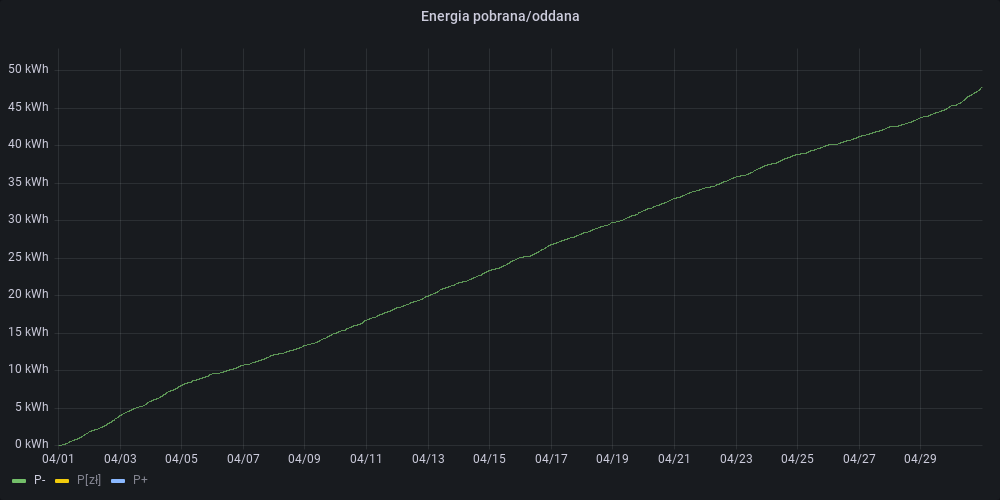
\includegraphics[width=1\textwidth]{gfx/ochotnica-dolna-atende-energy-consumed-produced}
 \caption{Energy consumption/production measured at an Energy Cluster member in Ochotnica Dolna, as shown on Grafana}
 \label{fig:chapter02:energydistribution}
\end{figure}
\begin{figure}[htbp]
 \centering
 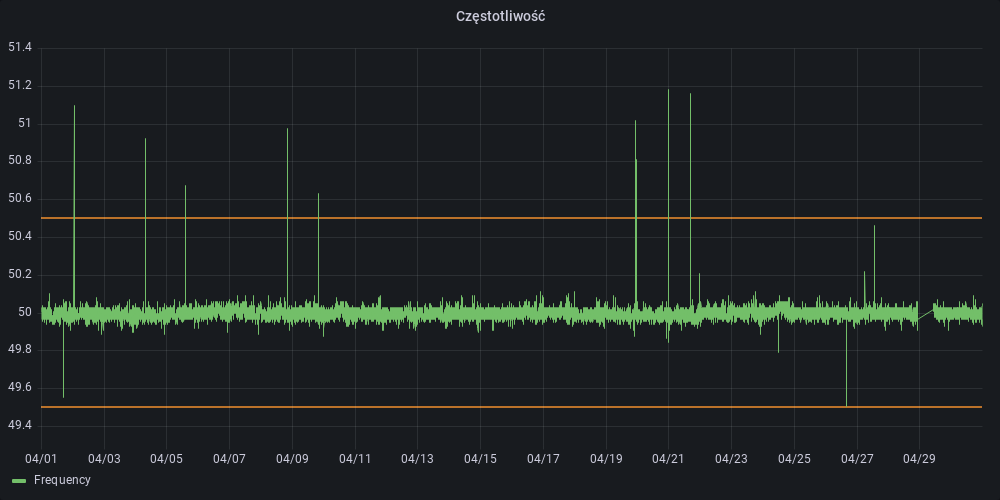
\includegraphics[width=1\textwidth]{gfx/ochotnica-dolna-atende-frequency}
 \caption{Frequency monitored at an Energy Cluster member in Ochotnica Dolna, as shown on Grafana}
 \label{fig:chapter02:energydistribution}
\end{figure}

\section{Performance analyses}

\par While all DBMSs can scale either vertically or horizontally. Every such improvement, however, is associated with higher costs. Performing basic \textbf{CRUD} operations is also essential in deciding on a specific DBMS since higher-performance databases require lower expenses when purchasing the hardware on which the database will operate.
\par For the purposes of this paper, python scripts capable of executing basic database operations, measuring the execution time, and drawing charts representing the results were written. 

\subsection{CRUD operations performing objects}
\par A python class was written for each considered DBMS to connect to these databases and perform basic operations on stored data. Every Class implementing this Interface must introduce four methods, each representing one of the four CRUD operations. Each of these methods must take two arguments: the amount of data created, read, updated, or deleted in a transaction or a batch operation and the number of transactions or batch operations performed. The Interface also defines a "reset()" operation that wipes leftover data from the database in preparation for performing the analysis and a "getName()" method that returns the name of the DBMS it performs the operations on, applicable when drawing charts.
\begin{lstlisting}[language=Python, caption=DatabaseTestingInterface]
from abc import ABC, abstractmethod
from typing import List, Dict, Tuple, Union
import csv
import itertools
from datetime import datetime

class DatabaseTestingInterface (ABC):
    @abstractmethod
    def create(self, rows_created: int = 1, transactions: int = 1):
        pass

    @abstractmethod
    def read(self, rows_read: int = 1, transactions: int = 1):
        pass

    @abstractmethod
    def update(self, rows_updated: int = 1, transactions: int = 1):
        pass

    @abstractmethod
    def delete(self, rows_deleted: int = 1, transactions: int = 1):
        pass

    @abstractmethod
    def reset(self):
        pass

    @abstractmethod
    def getName(self) -> str:
        pass
\end{lstlisting}
\par While not included inside the Interface definition, every database connection object should also define a constructor that establishes a connection with the database and processes external CSV files into data used in CRUD operations. They should also define a destructor that would finally sever the connection to the database upon the object's destruction. They also usually implement methods that help create necessary data storage structures, like tables or collections.
/listing{SQLiteCRUDConnection}
\begin{lstlisting}[language=Python, caption=SQLiteDatabaseTesting]
import sqlite3

class SqliteDatabaseTesting(DatabaseTestingInterface):
    def __init__(self, connection_string: str, csv_file_paths: List[str]):
        self.connection = sqlite3.connect(connection_string)
        self.csv_data = {}
        self.table_names = []
        self.table_column_names = {}

        for file_path in csv_file_paths:
            table_name = os.path.splitext(os.path.basename(file_path))[0]
            self.table_names.append(table_name)
            self.table_column_names[table_name], self.csv_data[table_name] = self.__parse_csv_data(file_path)

        self.__normalize_table_column_names()
        self.__create_tables()
        self.connection.commit()

    def __create_tables(self):
        c = self.connection.cursor()
        for table_name in self.table_names:
            c.execute(f"DROP TABLE IF EXISTS {table_name}")
            column_definitions = []
            column_definitions.append(f"{self.table_column_names[table_name][0]} timestamp NOT NULL")
            column_definitions.append(f"{self.table_column_names[table_name][1]} timestamp NOT NULL")
            column_definitions.append(f"{self.table_column_names[table_name][2]} numerical NOT NULL")
            column_definitions.append(f"{self.table_column_names[table_name][3]} int")
            column_definitions_str = ", ".join(column_definitions)
            c.execute(f"CREATE TABLE {table_name} ({column_definitions_str})")
        self.connection.commit()

    def __normalize_table_column_names(self):
        for table_name, column_names in self.table_column_names.items():
            column_names = [''.join(c for c in name.strip() if c.isalnum() or c == '_') for name in column_names]
            self.table_column_names[table_name] = column_names

    def __parse_csv_data(self, file_path: str) -> Tuple[List[str], List[Tuple[str, str, float, int]]]:
        MAX_DATA_READ = 1000
        with open(file_path, "r") as f:
            reader = csv.reader(f, delimiter="|")
            column_names = next(reader)
            rows = itertools.islice(reader, MAX_DATA_READ)
            data = [tuple(row) for row in rows]
        return column_names, data

    def create(self, rows_created: int = 1, transactions: int = 1):
        for table_name, data in self.csv_data.items():
            for transaction in range(transactions):
                c = self.connection.cursor()
                for i in range(rows_created):
                    c.execute(f"INSERT INTO {table_name} VALUES (?, ?, ?, ?)", data[i+transaction*rows_created])
                self.connection.commit()

    def read(self, rows_read: int = 1, transactions: int = 1):
        for table_name in self.table_names:
            for transaction in range(transactions):
                c = self.connection.cursor()
                c.execute(f"SELECT * FROM {table_name} LIMIT {rows_read}")
                c.fetchone()

    def update(self, rows_updated: int = 1, transactions: int = 1):
        for table_name in self.table_names:
            for transaction in range(transactions):
                c = self.connection.cursor()
                for i in range(rows_updated):
                    c.execute(f"UPDATE {table_name} SET {self.table_column_names[table_name][2]} = 0 WHERE {self.table_column_names[table_name][0]} = \"{self.csv_data[table_name][i+transaction*rows_updated][0]}\"")
                self.connection.commit()

    def delete(self, rows_deleted: int = 1, transactions: int = 1):
        for table_name in self.table_names:
            for transaction in range(transactions):
                c = self.connection.cursor()
                for i in range(rows_deleted):
                    c.execute(f"DELETE FROM {table_name} WHERE {self.table_column_names[table_name][0]} = \"{self.csv_data[table_name][i+transaction*rows_deleted][0]}\"")
                self.connection.commit()

    def reset(self):
        c = self.connection.cursor()
        c.execute("SELECT name FROM sqlite_master WHERE type='table';")
        table_names = [row[0] for row in c.fetchall()]
        for table_name in table_names:
            c.execute(f"DROP TABLE IF EXISTS {table_name}")
        self.connection.commit()
        self.__create_tables()

    def __del__(self):
        self.connection.close()

    def getName(self) -> str:
        return "SQLite"
\end{lstlisting}
\par The default SQLite interface is used to implement this Class. The constructor stores the connection to the database file, whose path was provided during the object's construction, and processes external CSV data into a dictionary containing lists of data values for each table separately. 
\par The structure of the tables that will contain these data entries is hardcoded because every data type is organized in a similar way.
/listing{PostgresCRUDConnection}
\begin{lstlisting}[language=Python, caption=PostgresDatabaseTesting]
import psycopg2

class PostgresDatabaseTesting(DatabaseTestingInterface):
    def __init__(self, connection_string: str, csv_file_paths: List[str]):
        self.connection = psycopg2.connect(connection_string)
        self.csv_data = {}
        self.table_names = []
        self.table_column_names = {}

        for file_path in csv_file_paths:
            table_name = os.path.splitext(os.path.basename(file_path))[0]
            self.table_names.append(table_name)
            self.table_column_names[table_name], self.csv_data[table_name] = self.__parse_csv_data(file_path)

        self.__normalize_table_column_names()
        self.__create_tables()

    def __create_tables(self):
        cursor = self.connection.cursor()
        for table_name in self.table_names:
            cursor.execute(f"DROP TABLE IF EXISTS {table_name}")
            column_definitions = []
            column_definitions.append(f"{self.table_column_names[table_name][0]} timestamp NOT NULL")
            column_definitions.append(f"{self.table_column_names[table_name][1]} timestamp NOT NULL")
            column_definitions.append(f"{self.table_column_names[table_name][2]} numeric NOT NULL")
            column_definitions.append(f"{self.table_column_names[table_name][3]} integer")
            column_definitions_str = ", ".join(column_definitions)
            cursor.execute(f"CREATE TABLE {table_name} ({column_definitions_str})")
        self.connection.commit()

    def __normalize_table_column_names(self):
        for table_name, column_names in self.table_column_names.items():
            column_names = [''.join(c for c in name.strip() if c.isalnum() or c == '_') for name in column_names]
            self.table_column_names[table_name] = column_names

    def __parse_csv_data(self, file_path: str) -> Tuple[List[str], List[Tuple[str, str, float, int]]]:
        MAX_DATA_READ = 1000
        with open(file_path, "r") as f:
            reader = csv.reader(f, delimiter="|")
            column_names = next(reader)
            rows = itertools.islice(reader, MAX_DATA_READ)
            data = []
            for row in rows:
                row[0] = row[0].replace(",", ".")
                row[1] = row[1].replace(",", ".")
                data.append(tuple(row))

        return column_names, data

    def create(self, rows_created: int = 1, transactions: int = 1):
        for table_name, data in self.csv_data.items():
            for transaction in range(transactions):
                cursor = self.connection.cursor()
                for i in range(rows_created):
                    cursor.execute(f"INSERT INTO {table_name} VALUES (%s, %s, %s, %s)", data[i+transaction*rows_created])
                self.connection.commit()

    def read(self, rows_read: int = 1, transactions: int = 1):
        for table_name in self.table_names:
            for transaction in range(transactions):
                cursor = self.connection.cursor()
                cursor.execute(f"SELECT * FROM {table_name} LIMIT {rows_read}")
                cursor.fetchone()

    def update(self, rows_updated: int = 1, transactions: int = 1):
        for table_name in self.table_names:
            for transaction in range(transactions):
                cursor = self.connection.cursor()
                for i in range(rows_updated):
                    cursor.execute(f"UPDATE {table_name} SET {self.table_column_names[table_name][2]} = 0 WHERE {self.table_column_names[table_name][0]} = %s", (self.csv_data[table_name][i+transaction*rows_updated][0],))
                self.connection.commit()

    def delete(self, rows_deleted: int = 1, transactions: int = 1):
        for table_name in self.table_names:
            for transaction in range(transactions):
                cursor = self.connection.cursor()
                for i in range(rows_deleted):
                    cursor.execute(f"DELETE FROM {table_name} WHERE {self.table_column_names[table_name][0]} = %s", (self.csv_data[table_name][i+transaction*rows_deleted][0],))
                self.connection.commit()

    def reset(self):
        cursor = self.connection.cursor()
        for table_name in self.table_names:
            cursor.execute(f"DROP TABLE {table_name}")
        self.connection.commit()
        self.__create_tables()

    def getName(self) -> str:
        return "PostgreSQL"

    def __del__(self):
        self.connection.close()
\end{lstlisting}
\par The PostgreSQL implementation is very similar to the SQLite implementation since the PostgreSQL handling library "psycopg2" uses the same basic syntax as the sqlite3 library. The main difference is in the structure of the connection string - while SQLite requires the path to the location of the database on disk, PostgreSQL needs a string of data that defines the IP address of the DBMS service, the database name, the user name, and password. 
/listing{Cassandra}
\begin{lstlisting}[language=Python, caption=CassandraDatabaseTesting]
import cassandra
from cassandra.cluster import Cluster
from cassandra.query import SimpleStatement, BatchStatement
from typing import List, Tuple

class CassandraDatabaseTesting(DatabaseTestingInterface):
    def __init__(self, connection_string: str, csv_file_paths: List[str]):
        self.cluster = Cluster([connection_string])
        self.session = self.cluster.connect()
        self.csv_data = {}
        self.table_names = []
        self.table_column_names = {}
        self.KEYSPACE_NAME = "databaseTesting"

        for file_path in csv_file_paths:
            table_name = os.path.splitext(os.path.basename(file_path))[0]
            self.table_names.append(table_name)
            self.table_column_names[table_name], self.csv_data[table_name] = self.__parse_csv_data(file_path)

        self.__normalize_table_column_names()
        self.__execute_simple_statement(f"DROP KEYSPACE IF EXISTS {self.KEYSPACE_NAME}")
        self.__create_tables()

    def __execute_simple_statement(self, query: str, parameters: Tuple = ()):
        statement = SimpleStatement(query, consistency_level=cassandra.ConsistencyLevel.ONE)
        self.session.execute(statement, parameters)

    def __execute_batch_statement(self, batch_type: str, statements: List[str], parameters_list: List[Tuple[Tuple]]):
        batch = BatchStatement(batch_type=batch_type, consistency_level=cassandra.ConsistencyLevel.ONE)
        for statement, parameters in zip(statements, parameters_list):
            batch.add(statement, parameters)
        self.session.execute(batch)

    def __create_tables(self):
        self.__execute_simple_statement(f"CREATE KEYSPACE {self.KEYSPACE_NAME} WITH REPLICATION = {{'class': 'SimpleStrategy', 'replication_factor': 1}}")
        self.__execute_simple_statement(f"USE {self.KEYSPACE_NAME}")
        for table_name in self.table_names:
            self.__execute_simple_statement(f"CREATE TABLE IF NOT EXISTS {table_name} ({self.table_column_names[table_name][0]} timestamp, {self.table_column_names[table_name][1]} timestamp, {self.table_column_names[table_name][2]} float, {self.table_column_names[table_name][3]} int, PRIMARY KEY ({self.table_column_names[table_name][0]}, {self.table_column_names[table_name][1]}))")

    def __normalize_table_column_names(self):
        for table_name, column_names in self.table_column_names.items():
            column_names = [''.join(c for c in name.strip() if c.isalnum() or c == '_') for name in column_names]
            self.table_column_names[table_name] = column_names

    def __parse_csv_data(self, file_path: str) -> Tuple[List[str], List[Tuple[str, str, float, int]]]:
        MAX_DATA_READ = 1000
        with open(file_path, "r") as f:
            reader = csv.reader(f, delimiter="|")
            column_names = next(reader)
            rows = itertools.islice(reader, MAX_DATA_READ)
            data = []
            for row in rows:
                row[0] = row[0].replace(",", ".")
                row[1] = row[1].replace(",", ".")
                data.append(tuple(row))

        return column_names, data

    def create(self, rows_created: int = 1, transactions: int = 1):
        for table_name, data in self.csv_data.items():
            for transaction in range(transactions):
                statements = []
                parameters_list = []
                for i in range(rows_created):
                    statements.append(f"INSERT INTO {table_name} ({self.table_column_names[table_name][0]}, {self.table_column_names[table_name][1]}, {self.table_column_names[table_name][2]}, {self.table_column_names[table_name][3]}) VALUES (%s, %s, %s, %s)")
                    parameters_list.append((data[i][0], data[i][1], float(data[i][2]), int(data[i][3])))

                self.__execute_batch_statement(batch_type=BatchStatement.Type.UNLOGGED, statements=statements, parameters_list=parameters_list)

    def read(self, rows_read: int = 1, transactions: int = 1):
        for table_name in self.table_names:
            for transaction in range(transactions):
                statement = f"SELECT * FROM {table_name} LIMT {rows_read}"
                self.session.execute(statement)

    def update(self, rows_updated: int = 1, transactions: int = 1):
        for table_name, data in self.csv_data.items():
            for transaction in range(transactions):
                statements = []
                parameters_list = []
                for i in range(rows_updated):
                    statements.append(f"UPDATE {table_name} SET {self.table_column_names[table_name][2]} = %s WHERE {self.table_column_names[table_name][0]} = %s AND {self.table_column_names[table_name][1]} = %s")
                    parameters_list.append((float(self.csv_data[table_name][i][2]), self.csv_data[table_name][i][0], self.csv_data[table_name][i][1]))

                self.__execute_batch_statement(batch_type=BatchStatement.Type.UNLOGGED, statements=statements, parameters_list=parameters_list)

    def delete(self, rows_deleted: int = 1, transactions: int = 1):
        for table_name, data in self.csv_data.items():
            for transaction in range(transactions):
                statements = []
                parameters_list = []
                for i in range(rows_deleted):
                    statements.append(f"DELETE FROM {table_name} WHERE {self.table_column_names[table_name][0]} = %s AND {self.table_column_names[table_name][1]} = %s")
                    parameters_list.append((self.csv_data[table_name][i][0], self.csv_data[table_name][i][1]))

                self.__execute_batch_statement(batch_type=BatchStatement.Type.UNLOGGED, statements=statements, parameters_list=parameters_list)

    def reset(self):
        self.__execute_simple_statement(f"DROP KEYSPACE {self.KEYSPACE_NAME}")
        self.__create_tables()

    def getName(self) -> str:
        return "Cassandra"

    def __del__(self):
        self.session.close()
\end{lstlisting}
\par The Cassandra version of this Class is also very similar to its SQL counterparts due to CQL's resemblance to SQL. The lack of transactions in Cassandra causes the main difference in implementation. Instead, the BatchStatement mechanism was used to perform multiple operations at once.
/listing{MongoDB}
\begin{lstlisting}[language=Python, caption=MongoDatabaseTesting]
from pymongo import MongoClient
from pymongo.operations import InsertOne, UpdateOne, DeleteOne

class MongoDatabaseTesting(DatabaseTestingInterface):
    def __init__(self, connection_string: str, csv_file_paths: List[str]):
        self.client = MongoClient(connection_string)
        self.csv_data = {}
        self.collection_names = []
        self.collection_column_names = {}
        self.DATABASE_NAME = "databasetesting"

        for file_path in csv_file_paths:
            collection_name = os.path.splitext(os.path.basename(file_path))[0]
            self.collection_names.append(collection_name)
            self.collection_column_names[collection_name], self.csv_data[collection_name] = self.__parse_csv_data(file_path)

        self.__normalize_collection_column_names()

    def __normalize_collection_column_names(self):
        for database_name, column_names in self.collection_column_names.items():
            column_names = [''.join(c for c in name.strip() if c.isalnum() or c == '_') for name in column_names]
            self.collection_column_names[database_name] = column_names

    def __parse_csv_data(self, file_path: str) -> Tuple[List[str], List[Tuple[str, str, float, int]]]:
        MAX_DATA_READ = 1000

        with open(file_path, "r") as f:
            reader = csv.reader(f, delimiter="|")
            column_names = next(reader)
            rows = itertools.islice(reader, MAX_DATA_READ)
            data = []
            for row in rows:
                row[0] = row[0].replace(",", ".")
                row[1] = row[1].replace(",", ".")
                data.append(tuple(row))

        return column_names, data

    def __convert_timestamp(self, timestamp_string: str):
        return datetime.strptime(timestamp_string, '%Y-%m-%d %H:%M:%S.%f').timestamp()

    def create(self, rows_created: int = 1, transactions: int = 1):
        for collection_name, data in self.csv_data.items():
            for transaction in range(transactions):
                requests = []
                for i in range(rows_created):
                    requests.append(InsertOne({
                        self.collection_column_names[collection_name][0]: self.__convert_timestamp(data[i][0]),
                        self.collection_column_names[collection_name][1]: self.__convert_timestamp(data[i][1]),
                        self.collection_column_names[collection_name][2]: data[i][2],
                        self.collection_column_names[collection_name][3]: data[i][3]
                    }))
                for collection_name in self.collection_names:
                    db = self.client[self.DATABASE_NAME]
                    collection = db[collection_name]
                    collection.bulk_write(requests, ordered=False)

    def read(self, rows_read: int = 1, transactions: int = 1):
        for collection_name in self.collection_names:
            db = self.client[self.DATABASE_NAME]
            collection = db[collection_name]
            for transaction in range(transactions):
                collection.find().limit(rows_read).next()

    def update(self, rows_updated: int = 1, transactions: int = 1):
        for collection_name, data in self.csv_data.items():
            for transaction in range(transactions):
                requests = []
                for i in range(rows_updated):
                    requests.append(UpdateOne({self.collection_column_names[collection_name][0]: self.__convert_timestamp(self.csv_data[collection_name][i][0]), self.collection_column_names[collection_name][1]: self.__convert_timestamp(self.csv_data[collection_name][i][1])}, {'$set': {self.collection_column_names[collection_name][2]: 0}}))
                for collection_name in self.collection_names:
                    db = self.client[self.DATABASE_NAME]
                    collection = db[collection_name]
                    collection.bulk_write(requests, ordered=False)

    def delete(self, rows_deleted: int = 1, transactions: int = 1):
        for collection_name, data in self.csv_data.items():
            for transaction in range(transactions):
                requests = []
                for i in range(rows_deleted):
                    requests.append(DeleteOne({self.collection_column_names[collection_name][0]: self.__convert_timestamp(self.csv_data[collection_name][i][0]), self.collection_column_names[collection_name][1]: self.__convert_timestamp(self.csv_data[collection_name][i][1])}))
                for collection_name in self.collection_names:
                    db = self.client[self.DATABASE_NAME]
                    collection = db[collection_name]
                    collection.bulk_write(requests, ordered=False)

    def reset(self):
        db = self.client[self.DATABASE_NAME]
        for collection_name in self.collection_names:
            db[collection_name].drop()

    def getName(self) -> str:
        return "MongoDB"

    def __del__(self):
        self.client.close()
\end{lstlisting}
\par The main difference in the MongoDB implementation is the use of documents to define data. There are no columns in document collections, so each document has to define the schema separately. The pymongo driver is also sensitive to the python data type of variables included in the document. Because of that, a method converting strings into timestamps was also defined within the Class.
\subsection{Evaluating performance}
\par A DatabaseTester Class was written to utilize these connection objects to measure the execution time of each operation. 
/listing{DatabaseTester}
\begin{lstlisting}[language=Python, caption=DatabaseTester]
from typing import List, Dict
import timeit
import matplotlib.pyplot as plt
import numpy as np

class DatabaseTester:
    def __init__(self, databaseList: List[DatabaseTestingInterface]):
        self.databaseList = databaseList
        self.executionTimeTable: List[List[Dict[int, float]]] = [[], [], [], []]
        for methodIndex in range(4):
            for _ in databaseList:
                self.executionTimeTable[methodIndex].append({})

    def testCreate(self, createdRecords: int = 1, recordsPerTransaction: int = 1):
        for databaseIndex, database in enumerate(self.databaseList):
            def prepeareCreate():
                database.reset()
            total_time = 0
            for currentRecord in range(0, createdRecords, recordsPerTransaction):
                print(f"inserting {currentRecord} of {createdRecords}")
                total_time += timeit.timeit(lambda: database.create(min(recordsPerTransaction, createdRecords - recordsPerTransaction)), lambda: prepeareCreate(), number=10)
            self.executionTimeTable[0][databaseIndex][recordsPerTransaction] = total_time

    def testRead(self, readRecords: int = 1, recordsPerTransaction: int = 1):
        for databaseIndex, database in enumerate(self.databaseList):
            database.reset()
            database.create(readRecords)
            total_time = 0
            for currentRecord in range(0, readRecords, recordsPerTransaction):
                print(f"reading {currentRecord} of {readRecords}")
                total_time += timeit.timeit(lambda: database.read(min(recordsPerTransaction, readRecords - recordsPerTransaction)), number=10)
            self.executionTimeTable[1][databaseIndex][recordsPerTransaction] = total_time

    def testUpdate(self, updatedRecords: int = 1, recordsPerTransaction: int = 1):
        for databaseIndex, database in enumerate(self.databaseList):
            def prepeareUpdate():
                database.reset()
                database.create(recordsPerTransaction)
            total_time = 0
            for currentRecord in range(0, updatedRecords, recordsPerTransaction):
                print(f"updating {currentRecord} of {updatedRecords}")
                total_time += timeit.timeit(lambda: database.update(min(recordsPerTransaction, updatedRecords - recordsPerTransaction)), lambda: prepeareUpdate(), number=10)
            self.executionTimeTable[2][databaseIndex][recordsPerTransaction] = total_time

    def tesetDelete(self, deletedRecords: int = 1, recordsPerTransaction: int = 1):
        for databaseIndex, database in enumerate(self.databaseList):
            def prepeareDelete():
                database.reset()
                database.create(recordsPerTransaction)
            total_time = 0
            for currentRecord in range(0, deletedRecords, recordsPerTransaction):
                print(f"deleting {currentRecord} of {deletedRecords}")
                total_time += timeit.timeit(lambda: database.delete(min(recordsPerTransaction, deletedRecords - recordsPerTransaction)), lambda: prepeareDelete(), number=10)
            self.executionTimeTable[3][databaseIndex][recordsPerTransaction] = total_time

    def drawGraphs(self):
        methodName = ['creating', 'reading', 'updating', 'deleting']
        for methodIndex, method in enumerate(self.executionTimeTable):
            labels = [database.getName() for database in self.databaseList]
            names = [x.__str__() for x in method[0].keys().__reversed__()]
            bar_width = 0.2
            bar_shift = bar_width

            x = np.arange(len(method[0].keys()))

            for i, database in enumerate(method):
                y = list(database.values().__reversed__())

                shift = ((-1*len(method)/2)*bar_width + bar_shift*i)

                plt.bar([xi + shift for xi in x], y, width=bar_width, label=labels[i])

            plt.xticks(x, names)
            plt.title(f'Time elapsed while {methodName[methodIndex]} a 1000 records.')
            plt.xlabel('Number of records per transaction')
            plt.ylabel('Elapsed Time (seconds)')
            plt.legend()
            plt.show()

    def setExecutionTimeTable(self, executionTimeTable):
        self.executionTimeTable = executionTimeTable

    def getExecutionTimeTable(self):
        return self.executionTimeTable
\end{lstlisting}
\par The constructor of this object requires providing a list of DatabaseCRUDConnection objects that will be used when performing the analysis. The "executionTimeTable" field provides storage for analysis results. There are four methods used to measure the execution time of basic CRUD operations. Each of these four methods requires two arguments: the number of records to be operated on and the number of transactions/batch operations used to perform said operations. The operation execution time is measured using the timeit library, and the result is recorded in the appropriate place inside the "executionTimeTable" field. The "drawGraphs()" method draws bar charts based on data stored inside the "executionTimeTable()" field.
\par This code was used to perform a performance analysis, with all database instances initiated on the same local machine, using docker virtualization. 
/{graphs}
\par The results suggest that database performance can be improved by sending data in batches. If lower-performing database equipment struggles to meet the demands of a large Energy Cluster, it may thus collect data at longer intervals.
\par Because of its paradigm's uniqueness, it was impossible to compare Prometheus to other databases. Prometheus does include the option to tune the data-scraping interval. Prometheus has been proven to handle large amounts of data inserts every second, enough to satisfy the needs of the largest Energy Clusters. \citep{prometheusSoundcloud}